%----------------------------------------------------------------------------------------
%	PACKAGES & THEMES
%----------------------------------------------------------------------------------------

\documentclass[8pt]{beamer}

\usepackage{etex}
\mode<presentation> {
\usetheme{Vilanova}
}

\usepackage[french]{babel}
\usepackage[utf8]{inputenc}
\usepackage{array}
\usepackage{graphicx}
\usepackage{booktabs}
\usepackage{amsmath,amssymb,amsthm}
\usepackage{xcolor}
\usepackage{tikz}
\usetikzlibrary{arrows}
\usepackage{pifont}
\usepackage{listings,color}

\definecolor{listcomment}{rgb}{0.0,0.5,0.0}
\definecolor{listkeyword}{rgb}{0.0,0.0,0.5}
\definecolor{listnumbers}{gray}{0.65}
\definecolor{listlightgray}{gray}{0.955}
\definecolor{listwhite}{gray}{1.0}

\AtBeginSection[]
{
\addtocounter{framenumber}{-1}
\begin{frame}
\frametitle{Sommaire}
\tableofcontents[currentsection]
\end{frame}}

%----------------------------------------------------------------------------------------
%	PAGE TITRE
%----------------------------------------------------------------------------------------
\title{Orfeo ToolBox}
\subtitle{Un logiciel libre pour le traitement d'images de télédétection (màj.  pour 6.2)}
\author{Equipe OTB}% date and event here
\date{}

\pgfdeclareimage[height=96mm,width=128mm]{background}{images/fondsClairSansLogo}
\pgfdeclareimage[height=0.2cm]{cc}{images/CC-licence.png}
\setbeamertemplate{background}{\pgfuseimage{background}}
\pgfdeclareimage[height=0.6cm]{logoIncrust}{images/logoIncrust}
\pgfdeclareimage[height=0.6cm]{OSGeo_logo}{images/OSGeo_logo}
\logo{
\begin{tabular}{p{0.22\textwidth}p{0.58\textwidth}p{0.1\textwidth}p{0.1\textwidth}}
\href{http://www.osgeo.org}{\pgfuseimage{OSGeo_logo}}
& \vspace{-0.03\textwidth} \scriptsize{} % date and event here
& \href{http://creativecommons.org/licenses/by-sa/3.0/}{\pgfuseimage{cc}} & \href{http://www.orfeo-toolbox.org}{\pgfuseimage{logoIncrust}}\\
\end{tabular}
}

\titlegraphic{\vspace*{-5em}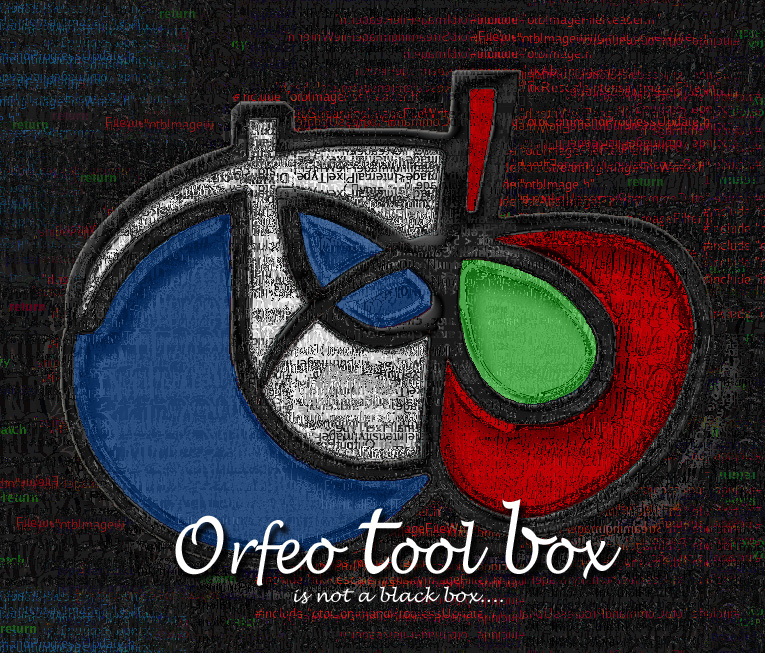
\includegraphics[width=.5\textwidth]{images/LOGOTB_blackbox.png}}

\begin{document}
\begin{frame}
\titlepage
\end{frame}

\section*{Introduction}

\begin{frame}
\frametitle{Si vous ne retenez qu'une planche\ldots}
\begin{block}{L'Orfeo ToolBox est:}
\begin{itemize}
\item Une \textbf{bibliothèque de traitement d'images} pour la télédétection
\item \textbf{Un logiciel libre} diffusé sous licence Apache v2.0 (depuis OTB 6.0, précédement CeCILL-v2)
\item \textbf{Financée et développée par le CNES} (principalement)
\item Projet OSGeo depuis 2017
\item Écrite en \textbf{C++} sur la base d'\href{www.itk.org}{ITK} (imagerie médicale)
\item Construite sur les épaules de géants (ITK, GDAL, OSSIM, OpenCV\ldots)
\item Conçue pour traiter de \textbf{gros volumes de données} de manière transparente grâce au traitement par morceaux et à la parallélisation
\end{itemize}
\end{block}

\begin{center}
{\huge\textcolor{red}{\href{http://www.orfeo-toolbox.org}{orfeo-toolbox.org}}}
\end{center}

\end{frame}

\begin{frame}
\frametitle{Pourquoi un logiciel libre ?}

\begin{block}{Diffusion maximale}
L'OTB est un logiciel à destination de tous les utilisateurs d'imagerie
spatiale. Sa diffusion large contribue au rayonnement des missions (Pléiades, Sentinels\ldots)
\end{block}

\begin{block}{Qualité et efficacité}
Le domaine fonctionnel de l'OTB est vaste, son développement nécessite du temps
et de l'expertise. L'ouverture des sources favorise:
\begin{itemize}
\item L'appropriation et la validation par la communauté des utilisateurs,
\item Les contributions et les corrections de bugs par les utilisateurs,
\item La dissémination sur de multiples plateformes.
\end{itemize}
\end{block}

\begin{block}{Démarche scientifique}
L'OTB capitalise une partie de la R\&D du CNES en extraction d'information, l'ouverture des sources permet une démarche de \textbf{recherche reproductible}.
\end{block}

\end{frame}

\section{Fonctionnalités}

\begin{frame}
\frametitle{Les grandes familles de fonctionnalités dans l'OTB (forcément incomplètes)}

\begin{block}{Pré-traitements}
\begin{itemize}
\item Calibration radiométrique, ortho-rectification, reprojection (raster et vecteur), pan-sharpening, stéréo-rectification,
\item Capteurs supportés: Sentinels, Pléiades, SPOT6, SPOT5, capteurs DigitalGlobe
\item Modélisation géométrique fournie par OSSIM, support de MNT SRTM ou GeoTIFF
\end{itemize}
\end{block}

\begin{block}{Manipulation d'images et de vecteurs}
\begin{itemize}
\item Formats supportés par Gdal (raster et vecteur), conversion raster/vecteur
\item Extraction de ROI, de bandes spectrales, concaténation ou séparation des bandes spectrales,
\item calcul mathématiques entre bandes, color mapping, optimisation du contraste
\item Filtrage linéaire, morphologie mathématique,
\end{itemize}
\end{block}
\end{frame}

\begin{frame}
\frametitle{Les grandes familles de fonctionnalités dans l'OTB (forcément incomplète)}

\begin{block}{Détection d'éléments saillants et calcul de primitives}
\begin{itemize}
\item Détection de contours, points d'intérêt SIFT et SURF, lignes, angles droits
\item Indices radiométriques, indices de textures (Haralick, SFS, PanTex)
\item Descripteurs statistiques locaux (moments de Flusser, HOG)
\item Matching de points d'intérêts
\end{itemize}
\end{block}

\begin{block}{Détection de changement}
\begin{itemize}
\item Algorithme classique avec métrique de comparaison d'images,
\item Algorithme MAD (Multivariate Alteration Detector)
\end{itemize}
\end{block}

\begin{block}{Réduction de la dimension, traitement hyperspectraux}
\begin{itemize}
\item Réduction de la dimension: PCA, NAPCA, ICA, MAF \ldots
\item Estimation de la dimension et extraction des pixels purs: algorithme VCA
\end{itemize}
\end{block}

\end{frame}

\begin{frame}
\frametitle{Les grandes familles de fonctionnalités dans l'OTB (forcément incomplète)}
\begin{block}{Segmentation}
\begin{itemize}
\item Algorithmes de segmentation Connected Components, MeanShift, Ligne de partage des eaux
\item Méthodologie pour une application large échelle,
\item Représentation vectorielles et raster des résultats, avec capacités d'analyse objet
\end{itemize}
\end{block}

\begin{block}{Classification}
\begin{itemize}
\item Supervision et classification d'images avec 9 algorithmes au choix (dont SVM et forêts aléatoires)
\item Fusion et régularisation de cartes de classification
\item Clustering de type K-Means ou carte de Kogonen
\item Classification objets (segments issus d'une segmentation)
\end{itemize}
\end{block}

\end{frame}

\vspace*{-6.5mm}
\begin{frame}[plain]
\hspace*{-11mm}
    \includegraphics[keepaspectratio,height=1.1\paperheight]{images/mayotte2012.png}
\end{frame}

\vspace*{-6.5mm}
\begin{frame}[plain]
\hspace*{-11mm}
    \includegraphics[keepaspectratio,height=1.1\paperheight]{images/mayotte2013.png}
\end{frame}

\vspace*{-6.5mm}
\begin{frame}[plain]
\hspace*{-11mm}
    \includegraphics[keepaspectratio,height=1.1\paperheight]{images/mayotte_mad.png}
\end{frame}

\vspace*{-6.5mm}
\begin{frame}[plain]
\hspace*{-11mm}
\includegraphics[keepaspectratio,height=1.1\paperheight]{images/saint_paul_lsd.png}
\end{frame}

\vspace*{-6.5mm}
\begin{frame}[plain]
\hspace*{-11mm}
    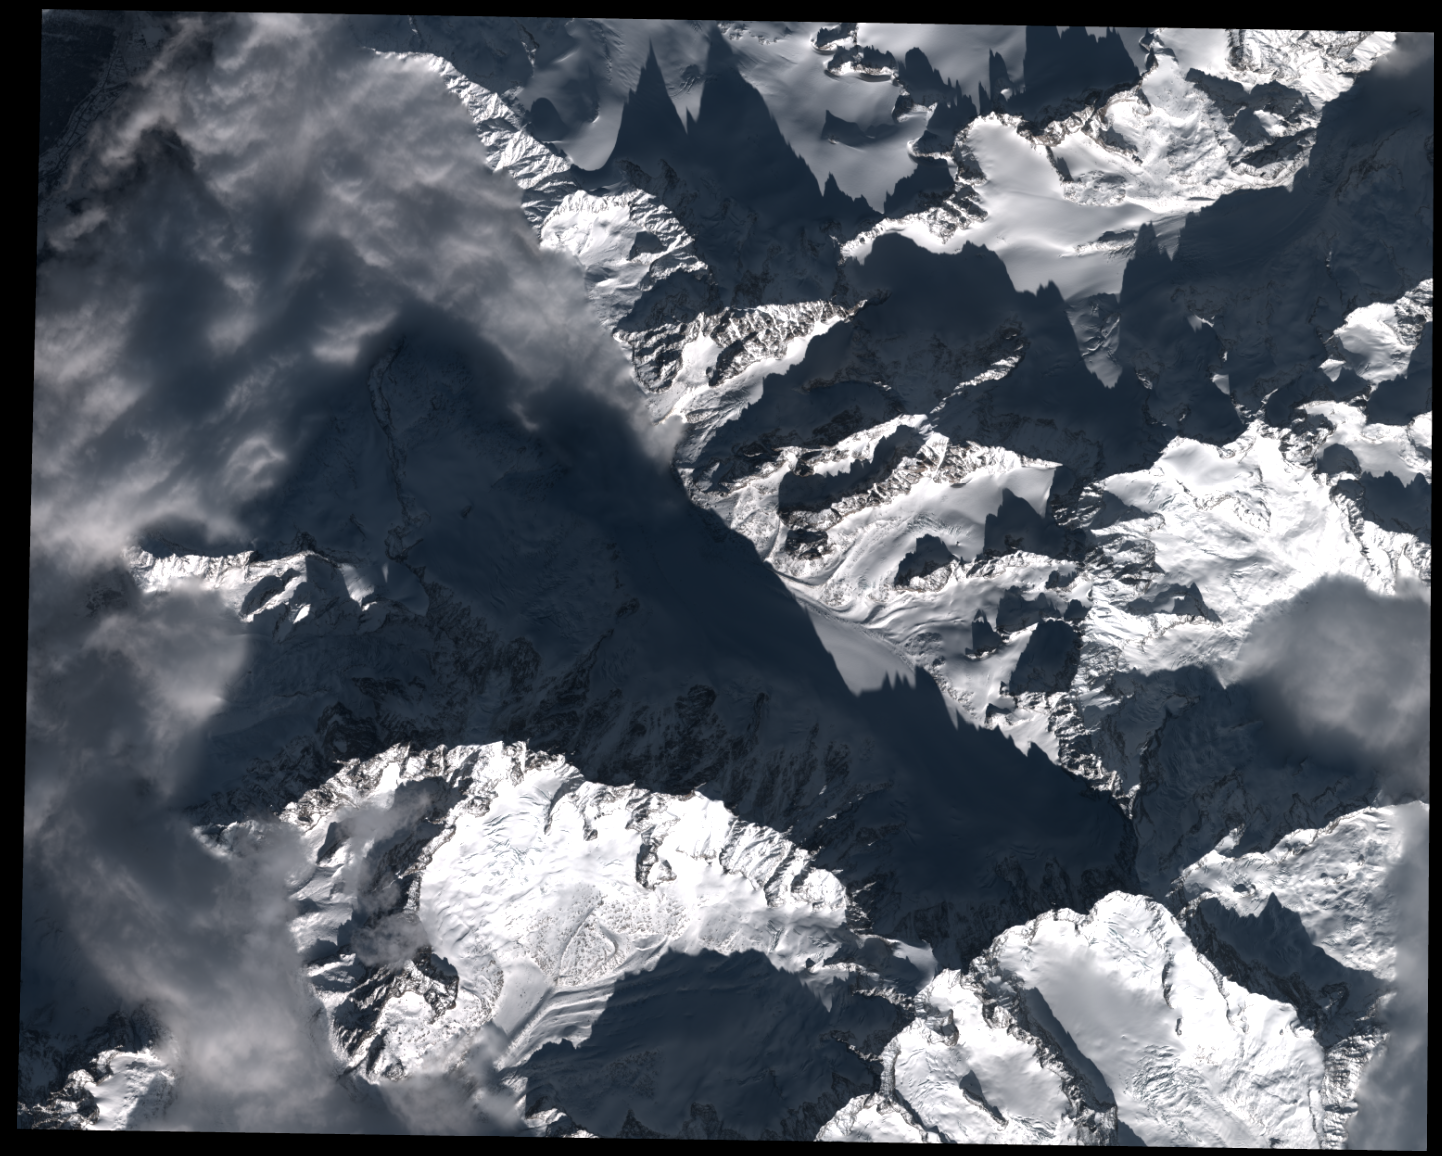
\includegraphics[keepaspectratio,width=1.005\paperwidth,height=1.1\paperheight]{images/argentiere_left.png}
\end{frame}

\vspace*{-6.5mm}
\begin{frame}[plain]
\hspace*{-11mm}
    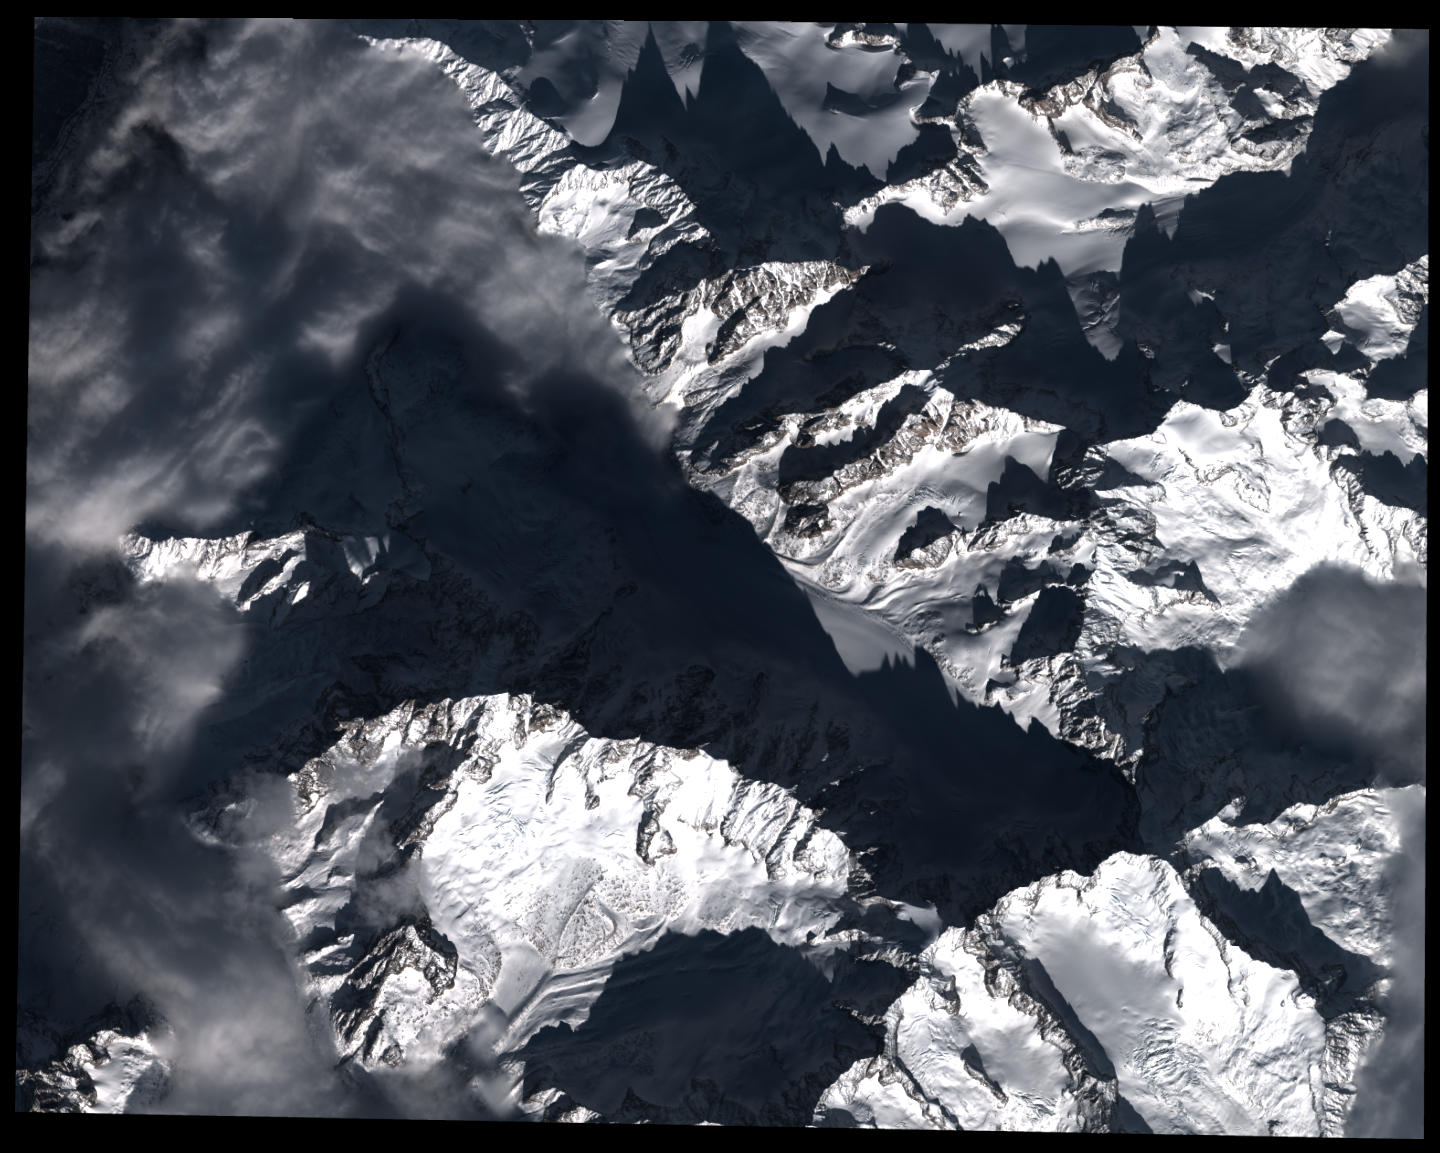
\includegraphics[keepaspectratio,width=1.005\paperwidth,height=1.1\paperheight]{images/argentiere_right.png}
\end{frame}

\vspace*{-6.5mm}
\begin{frame}[plain]
\hspace*{-11mm}
    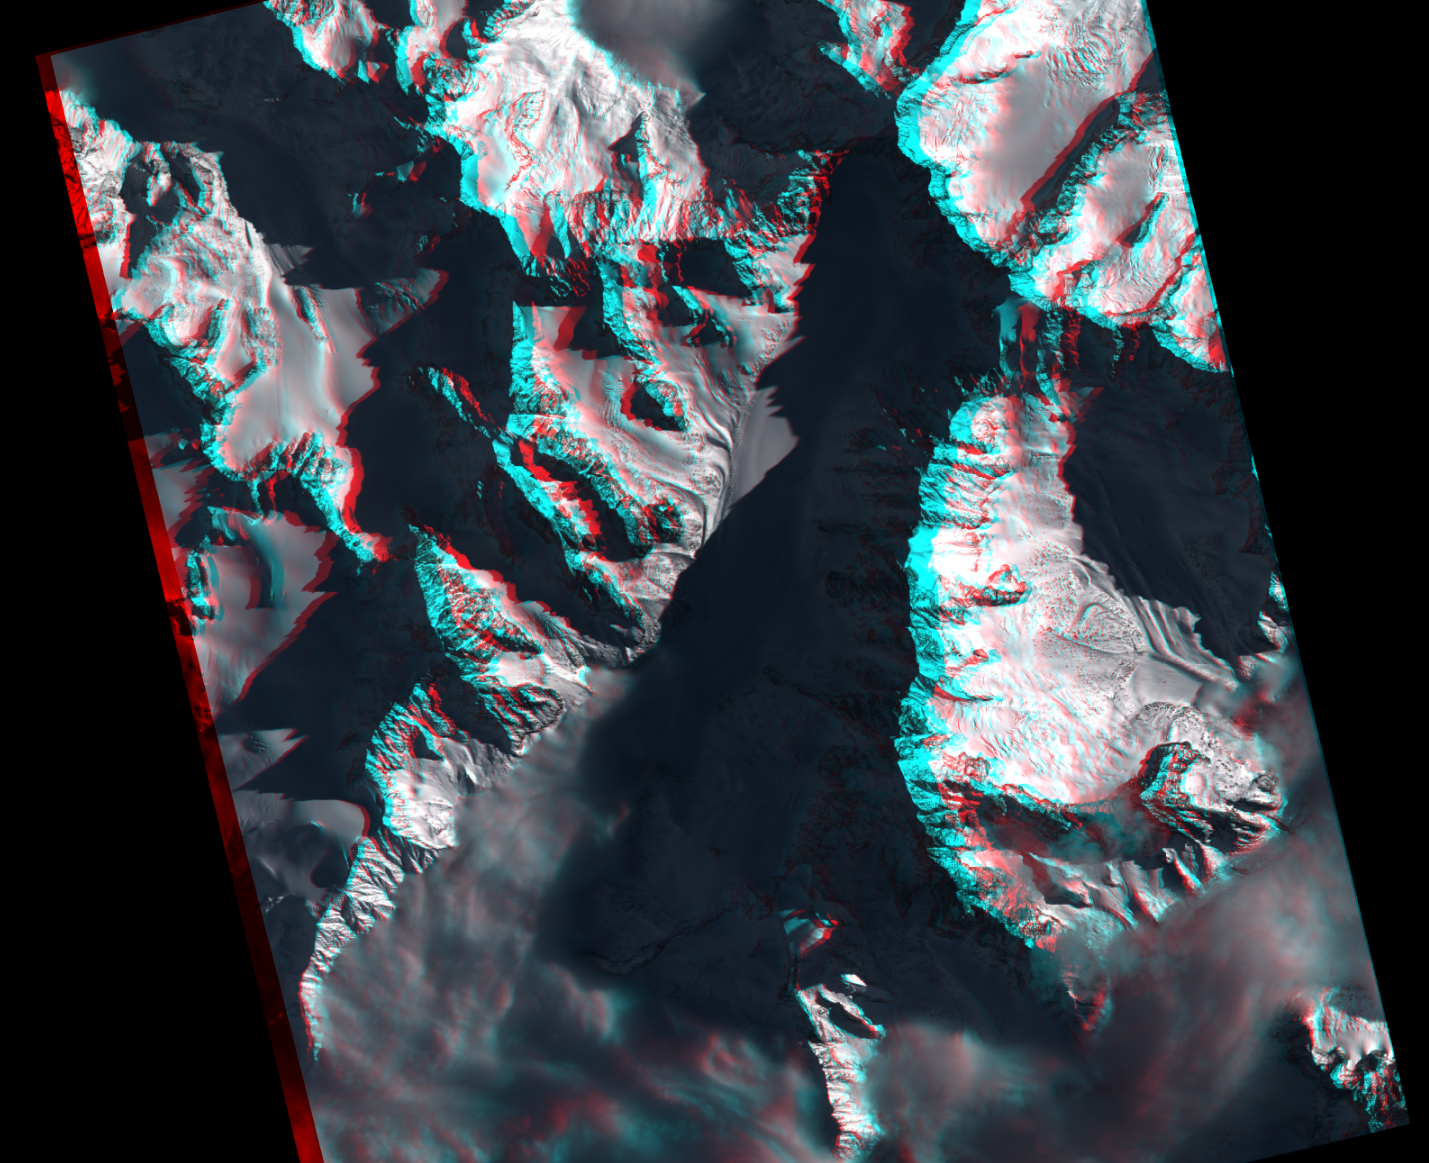
\includegraphics[keepaspectratio,width=1.005\paperwidth,height=1.1\paperheight]{images/argentiere_anaglyphe.png}
\end{frame}

\vspace*{-6.5mm}
\begin{frame}[plain]
\hspace*{-11mm}
    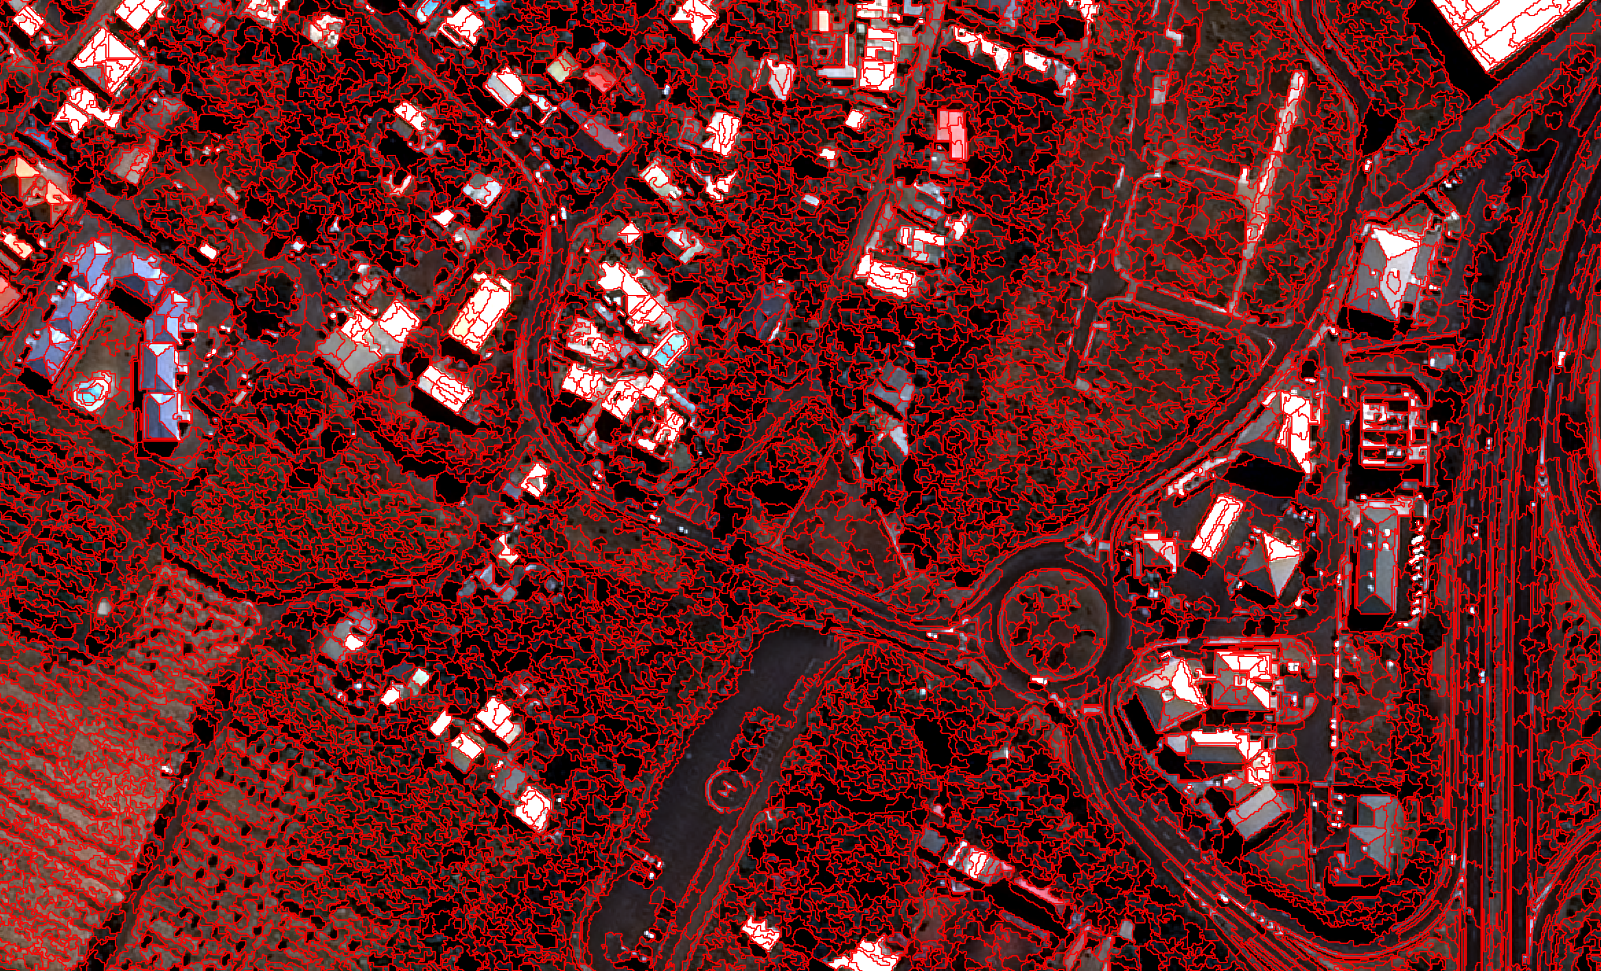
\includegraphics[keepaspectratio,height=1.1\paperheight]{images/segmentation.png}
\end{frame}

\vspace*{-6.5mm}
\begin{frame}[plain]
\hspace*{-11mm}
    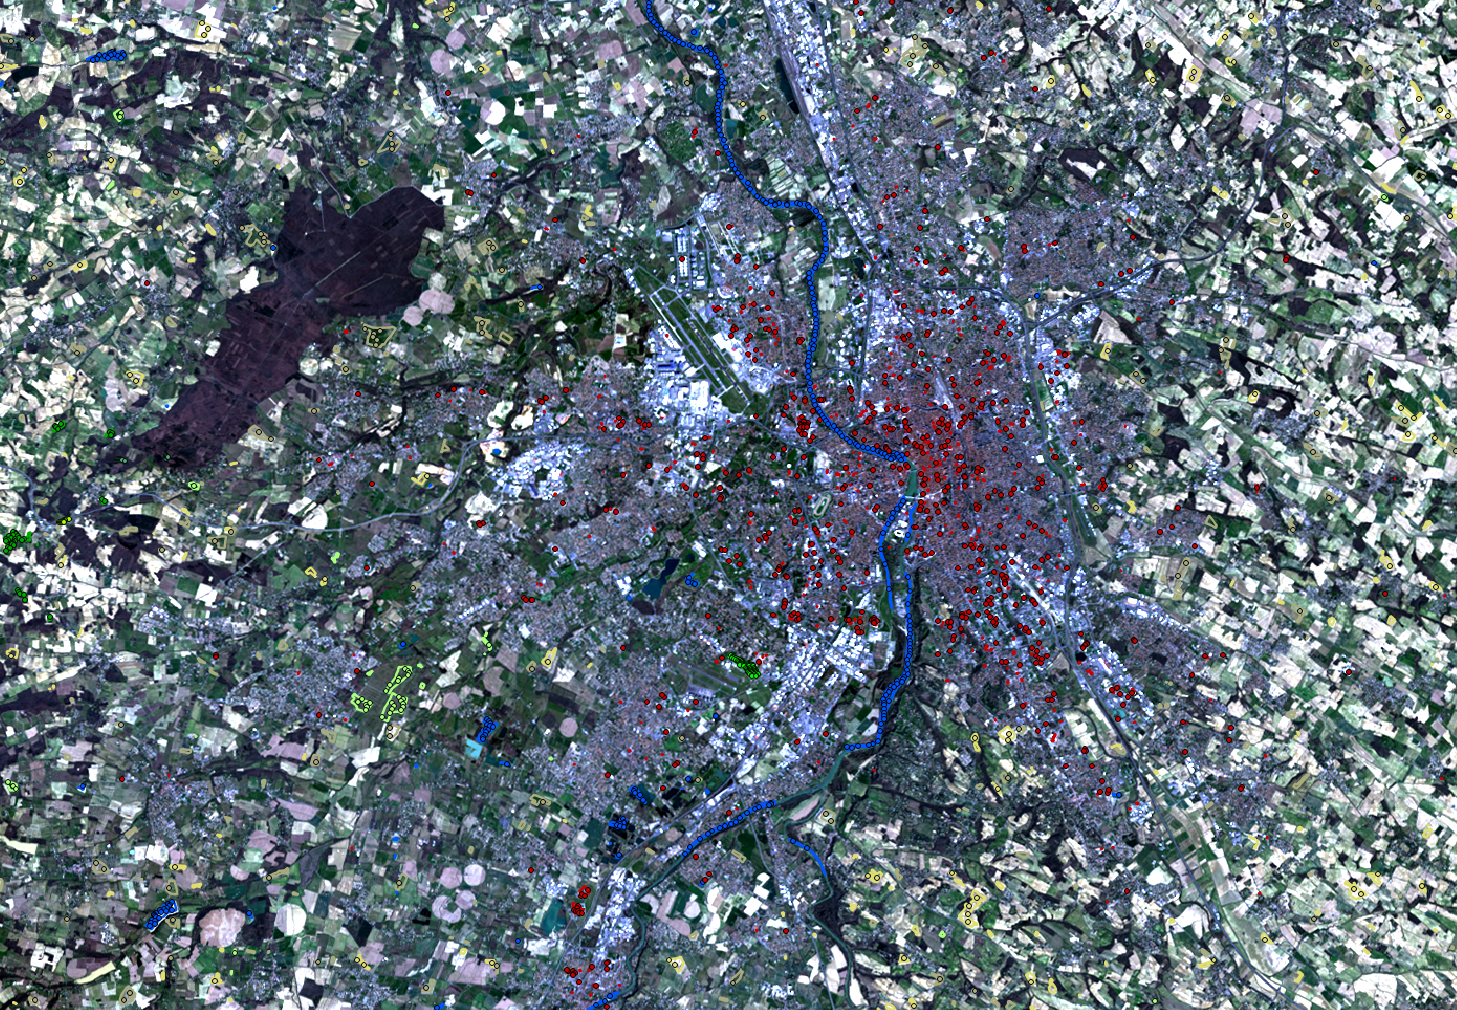
\includegraphics[keepaspectratio,height=1.1\paperheight]{../../Courses/org/WorkshopGuide/Images/samples_selection.png}
\end{frame}


\vspace*{-6.5mm}
\begin{frame}[plain]
\hspace*{-11mm}
    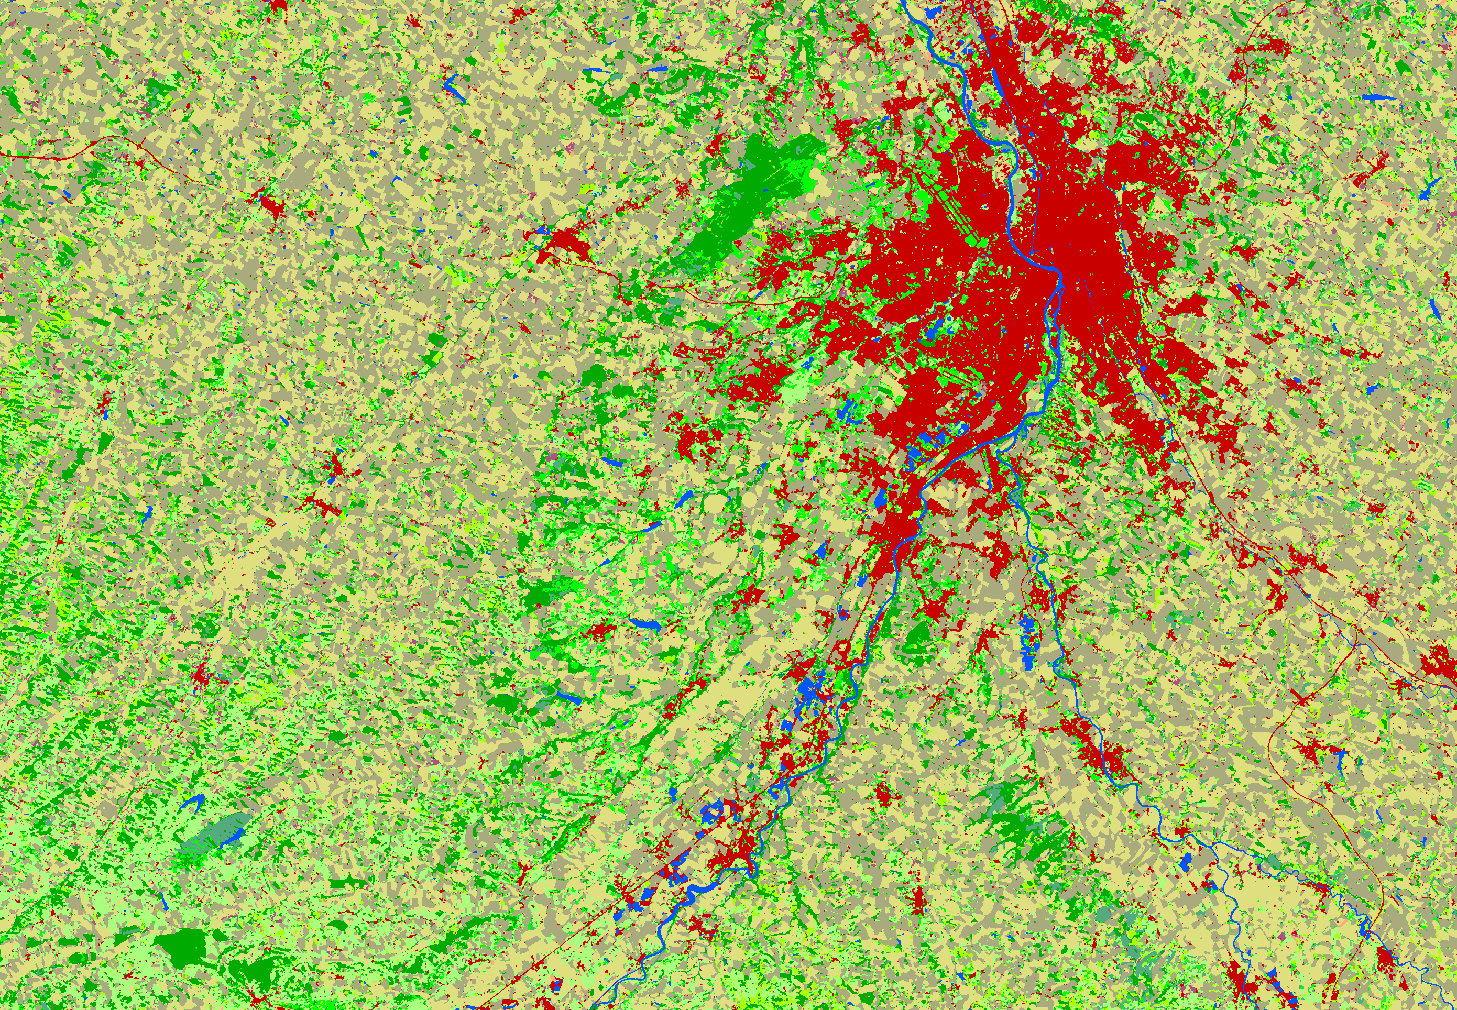
\includegraphics[keepaspectratio,height=1.1\paperheight]{../../Courses/org/WorkshopGuide/Images/final_classification.png}
\end{frame}

\section{Caractéristiques clés}

\begin{frame}
\frametitle{Construite sur des logiciels libres tiers performants}
\begin{block}{Motivations}
\begin{itemize}
\item A chaque fois que c'est possible, l'Orfeo ToolBox s'appuie sur des
  logiciels libres tiers
\item Cette position d'intégrateur permet d'accroître rapidement le nombre de fonctions tout en assurant leurs validité
\item Elle permet également de créer de nouvelles fonctionnalités par hybridation
\end{itemize}
\end{block}

\begin{block}{Les logiciels tiers principaux}
\begin{itemize}
\item \href{www.itk.org}{ITK}: modélisation de la chaîne de traitement
\item \href{www.gdal.org}{GDAL}: accès aux données images et vecteurs,
\item \href{www.ossim.org}{OSSIM}: modélisation géométrique des prises de vues,
\item \href{www.opencv.org}{OpenCV} et \href{www.libsvm.org}{LibSVM}: fonctionnalités de classification supervisée,
\item \href{www.muparser.org}{MuParser} et \href{www.muparserx.org}{MuParserX}:
analyse dynamique d'expressions mathématiques.
\end{itemize}
\end{block}


\end{frame}

\begin{frame}
\frametitle{Compatible (et disponible) pour un maximum de plateformes}
\begin{columns}
\column{0.5\textwidth}
\begin{block}{Objectif multi-plateforme}
\begin{itemize}
\item Compiler avec les versions récentes de:
\begin{itemize}
\item GCC
\item Clang
\item MinGW
\item Visual Studio\ldots
\end{itemize}
\item Des paquets binaires sont disponibles en fonction de la plateforme:
\begin{itemize}
\item Dépôt UbuntuGIS pour Ubuntu,
\item Intégration à OSGeo4W et paquets indépendants pour Windows,
\item Paquets MacPort, formule HomeBrew et image dmg pour Mac OS X\ldots
\end{itemize}
\end{itemize}
\end{block}
\column{0.5\textwidth}
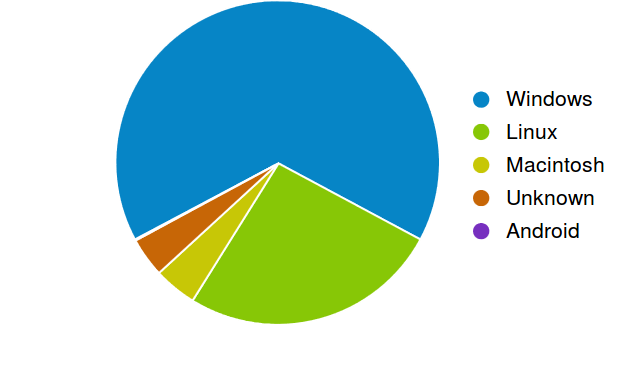
\includegraphics[width=\textwidth]{images/OTB4_download_sourceforge_os_crop.png}
\begin{center}
\tiny{Système d'exploitation des téléchargements sur Sourceforge (ne tient pas compte des autres dépôt)}
\end{center}
\end{columns}
\end{frame}

\begin{frame}
\frametitle{Flexibilité, passage à l'échelle: \textit{Pipeline}, \textit{Streaming} et \textit{multithreading}}

\begin{block}{Le modèle de \textit{Pipeline}}
\begin{center}
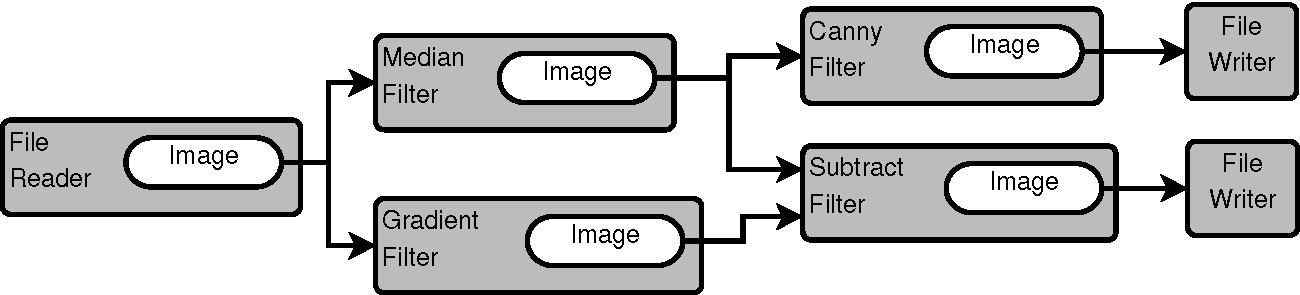
\includegraphics[width=0.7\textwidth]{images/ProcessObjectDataObject.png}
\end{center}
\end{block}
\vspace{-0.5cm}
\begin{block}{\textit{Streaming}}
\begin{center}
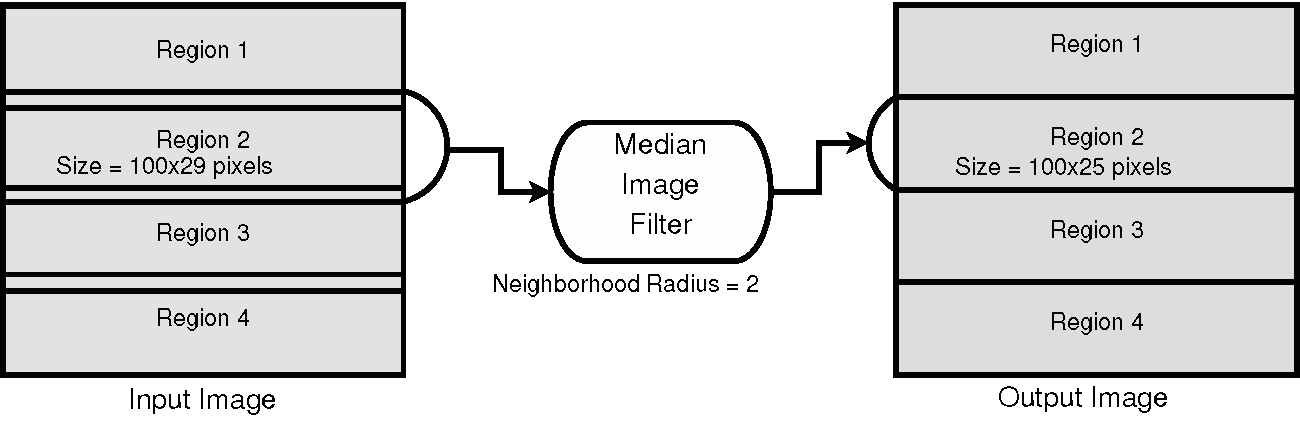
\includegraphics[width=0.7\textwidth]{images/StreamingImageDiagram.png}
\end{center}
\end{block}
\vspace{-0.5cm}
\begin{center}
\tiny{source: http://www.aosabook.org/en/itk.html}
\end{center}
\end{frame}

\begin{frame}
\frametitle{Flexibilité, passage à l'échelle: en coulisse ...}
\begin{center}
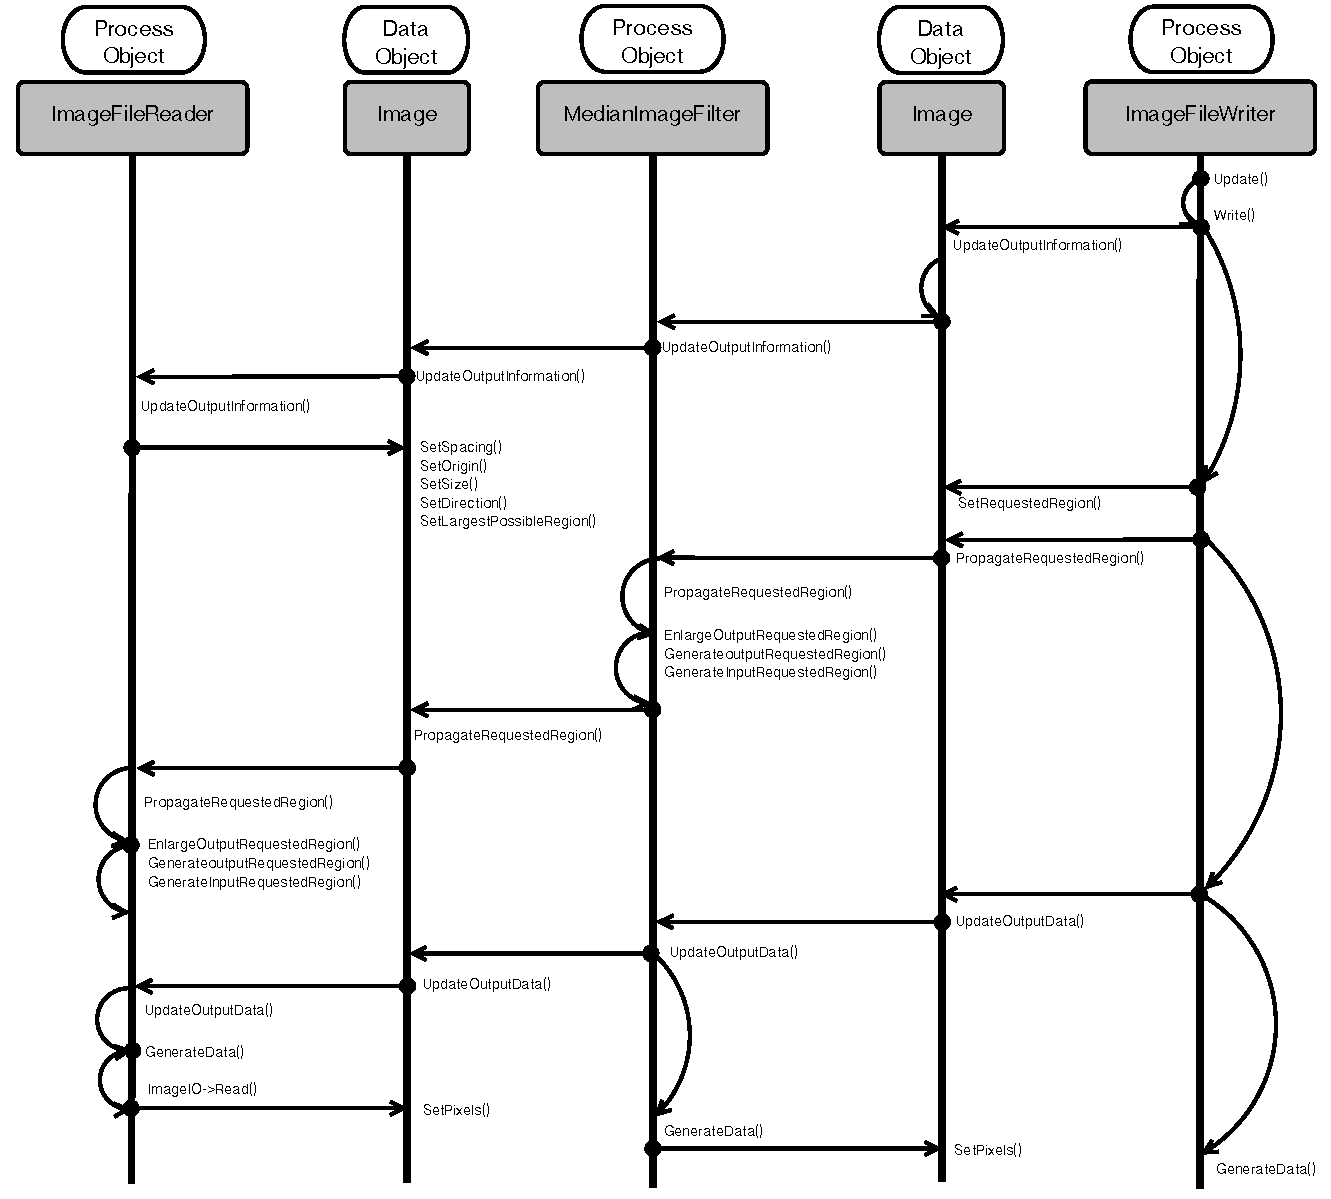
\includegraphics[width=0.6\textwidth]{images/ProcessObjectDataObjectInteractionUML.png}\\
\tiny{source: http://www.aosabook.org/en/itk.html}
\end{center}
\end{frame}

\begin{frame}
\frametitle{Proche de l'état de l'art}
\begin{itemize}
\item Veille technologique de l'équipe de développement
\item Implémentations d'algorithmes récents d'après publication. Ex.: profils morphologiques, segmentation MeanShift, textures de Haralick, points d'intérêt SURF \ldots
\item Implémentations de références contribuées par les auteurs de certains travaux en support à leur publication. Ex.: Large Scale MeanShift, fusion bayésienne, détection d'objets \ldots
\item Veille pour bénéficier des avancées des logiciels tiers. Ex.: algorithmes de \textit{machine learning} d'OpenCV,
\item Souvent: pour une même brique fonctionnelle, plusieurs algorithmes de complexités différentes disponibles sous une même interface.
\end{itemize}
\end{frame}


\begin{frame}
\frametitle{Un mot concernant le développement du logiciel}
\vspace{-0.5cm}
\begin{itemize}
\item Gestion de code source décentralisée: Git (migration depuis Mercurial en
  Juillet 2015)
\item C++ et suite CMake (CTest, CDash)
\item Développement guidé par les tests (TDD)
\item Gestion Agile (scrum)
\item Intégration continue et packaging automatisé
\end{itemize}
Tout les jours, environ 3000 tests sont compilés et rejoués sur 16
configurations différentes.
\begin{center}
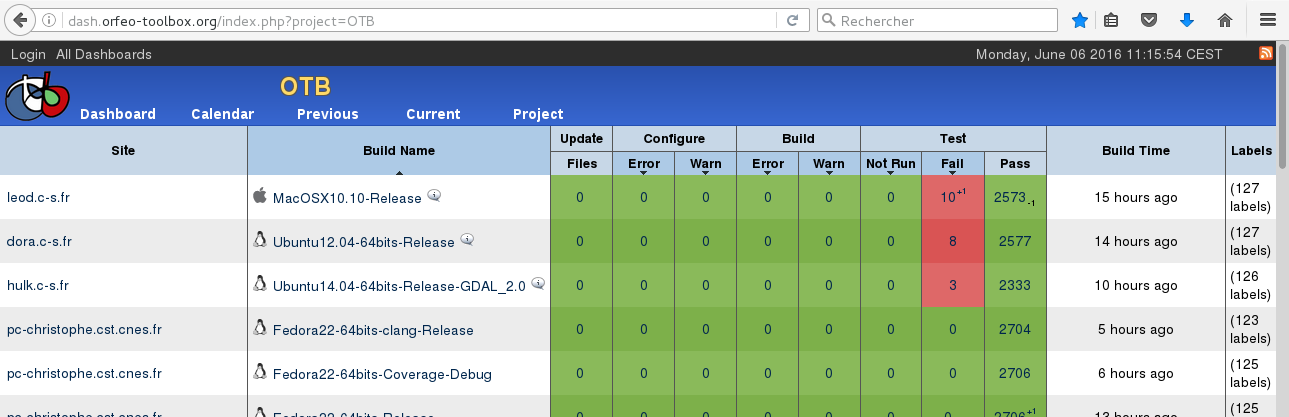
\includegraphics[width=\textwidth]{images/dashboard.png}
\end{center}
\end{frame}

\section{Comment utiliser OTB?}

\begin{frame}
\frametitle{Comment utiliser l'OTB?}
\vspace{-0.5cm}
\begin{center}
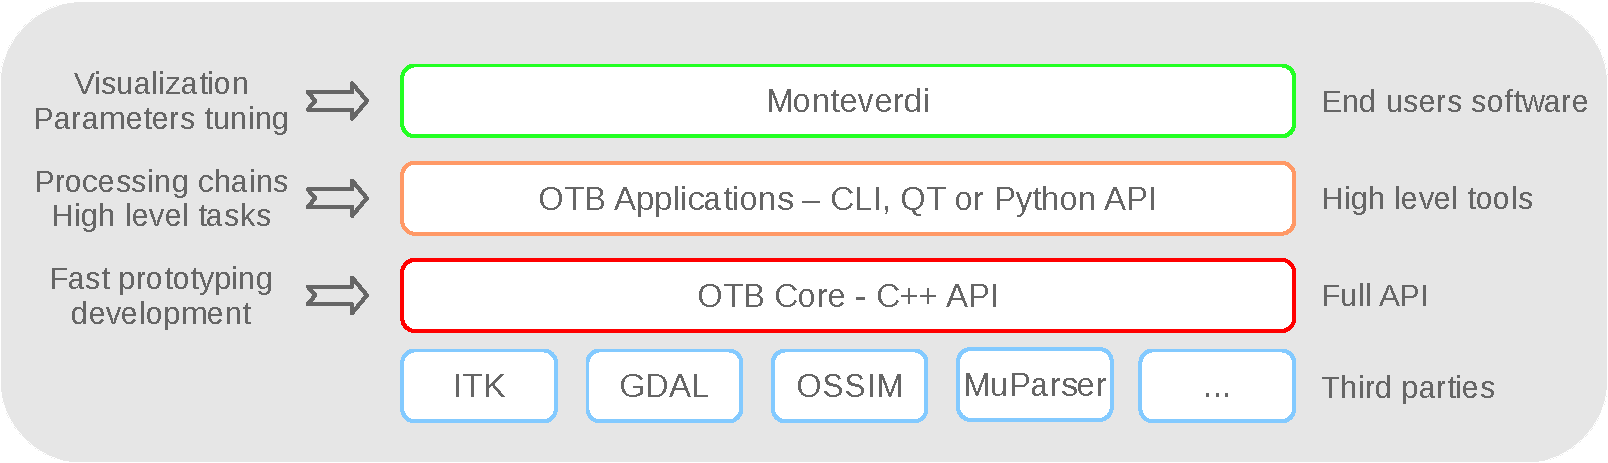
\includegraphics[width=\textwidth]{images/sandwich.pdf}
\end{center}
\vspace{-0.5cm}
\begin{block}{Écrire son propre code}
 Flexible, accès à l'API complète, demande une connaissance en C++
\end{block}
\begin{block}{Utiliser les applications}
 Fonctions de haut niveau (par ex. segmentation), appel en ligne de commande, via une interface graphique, ou depuis Python. Peut être étendue (création d'applications)
\end{block}
\begin{block}{Utiliser Monteverdi}
Visualisation, gestion persistante des données, \textcolor{red}{Accès à l'ensemble des applications}
\end{block}
\end{frame}

\begin{frame}[fragile]
\frametitle{Show me the code!}
\begin{lstlisting}[language=c++,breaklines=true,breakatwhitespace=true,frame = tb,framerule = 0.25pt,fontadjust,backgroundcolor={\color{listlightgray}},basicstyle = {\ttfamily\tiny},keywordstyle = {\ttfamily\color{listkeyword}\textbf},identifierstyle = {\ttfamily},commentstyle = {\ttfamily\color{listcomment}\textit},stringstyle = {\ttfamily},showstringspaces = false,showtabs = false,numbers = none,numbersep = 2pt, numberstyle={\ttfamily\color{listnumbers}},tabsize = 2]
#include "otbImage.h"
#include "otbImageFileReader.h"
#include "otbImageFileWriter.h"
#include "itkCannyEdgeDetectionImageFilter.h"
#include "itkRescaleIntensityImageFilter.h"

int main(int argc, char * argv[])
{
  typedef double                      PixelType;
  typedef otb::Image<PixelType>       ImageType;

  typedef unsigned char               OutputPixelType;
  typedef otb::Image<OutputPixelType> OutputImageType;

  typedef otb::ImageFileReader<ImageType> ReaderType;
  ReaderType::Pointer reader = ReaderType::New();

  reader->SetFileName(argv[1]);

  typedef itk::CannyEdgeDetectionImageFilter
  <ImageType, ImageType> FilterType;
  FilterType::Pointer filter = FilterType::New();

  filter->SetInput(reader->GetOutput());

  typedef otb::ImageFileWriter<OutputImageType> WriterType;
  WriterType::Pointer writer = WriterType::New();

  writer->SetFileName(argv[2]);

  writer->SetInput(filter->GetOutput());

  writer->Update();
}
\end{lstlisting}
\end{frame}

\begin{frame}
\frametitle{Les applications: codées une fois, utilisables partout}
\begin{columns}
\column{0.5\textwidth}
\begin{itemize}
\item 87 applications sont livrées avec l'OTB
\item 1 application $=$ 1 librairie dynamique (plugin)
\item Les applications sont auto-descriptives et auto-documentées
\item Les applications peuvent être étendues en dehors de l'OTB
\item Plusieurs interfaces sont disponibles pour utiliser les plugins:
\begin{itemize}
  \item Ligne de commande
  \item Interface Qt auto-générée
  \item Python
\end{itemize}
\item Les applications sont conçues pour une intégration facilitée dans des systèmes externes
\end{itemize}
\column{0.5\textwidth}
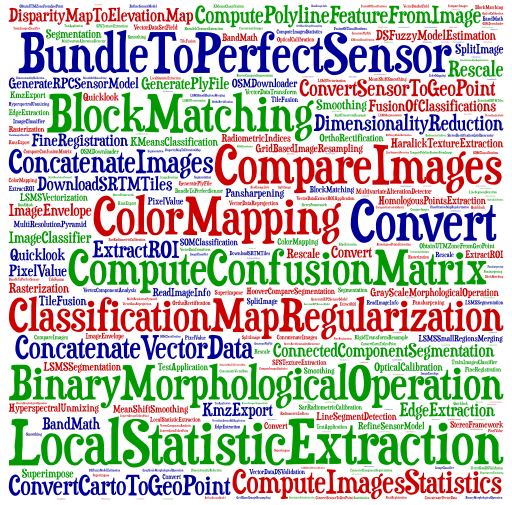
\includegraphics[width=\textwidth]{images/cloud_applications.png}
\end{columns}
\end{frame}



\begin{frame}[fragile]
\frametitle{Applications: appel depuis la ligne de commande}
\begin{scriptsize}
\vspace{-0.5cm}\begin{verbatim}
$ otbcli_OrthoRectification

ERROR: Waiting for at least one parameter...
This is the OrthoRectification application, version 5.2.1
This application allows to ortho-rectify optical images from supported sensors.

Complete documentation: http://www.orfeo-toolbox.org/Applications/OrthoRectification.html

Parameters:
        -progress                <boolean>        Report progress
MISSING -io.in                   <string>         Input Image  (mandatory)
MISSING -io.out                  <string> [pixel] Output Image  [pixel=uint8/uint16/int16/uint32/int32/float/double] (default value is float) (mandatory)
        -map                     <string>         Output Cartographic Map Projection [utm/lambert2/lambert93/wgs/epsg] (mandatory, default value is utm)
        -map.utm.zone            <int32>          Zone number  (mandatory, default value is 31)
        -map.utm.northhem        <boolean>        Northern Hemisphere  (optional, off by default)
        -map.epsg.code           <int32>          EPSG Code  (mandatory, default value is 4326)
        -outputs.mode            <string>         Parameters estimation modes [auto/autosize/autospacing/outputroi/orthofit] (mandatory, default value is auto)
MISSING -outputs.ulx             <float>          Upper Left X  (mandatory)
MISSING -outputs.uly             <float>          Upper Left Y  (mandatory)
MISSING -outputs.sizex           <int32>          Size X  (mandatory)
MISSING -outputs.sizey           <int32>          Size Y  (mandatory)
MISSING -outputs.spacingx        <float>          Pixel Size X  (mandatory)
MISSING -outputs.spacingy        <float>          Pixel Size Y  (mandatory)
        -outputs.lrx             <float>          Lower right X  (optional, off by default)
        -outputs.lry             <float>          Lower right Y  (optional, off by default)
        -outputs.ortho           <string>         Model ortho-image  (optional, off by default)
        -outputs.isotropic       <boolean>        Force isotropic spacing by default  (optional, on by default)
        -outputs.default         <float>          Default pixel value  (optional, on by default, default value is 0)
        -elev.dem                <string>         DEM directory  (optional, off by default)
        -elev.geoid              <string>         Geoid File  (optional, off by default)
        -elev.default            <float>          Default elevation  (mandatory, default value is 0)
        -interpolator            <string>         Interpolation [bco/nn/linear] (mandatory, default value is bco)
\end{verbatim}
\end{scriptsize}
\end{frame}

\begin{frame}[fragile]
\frametitle{Applications OTB: Interface graphique}
\begin{center}
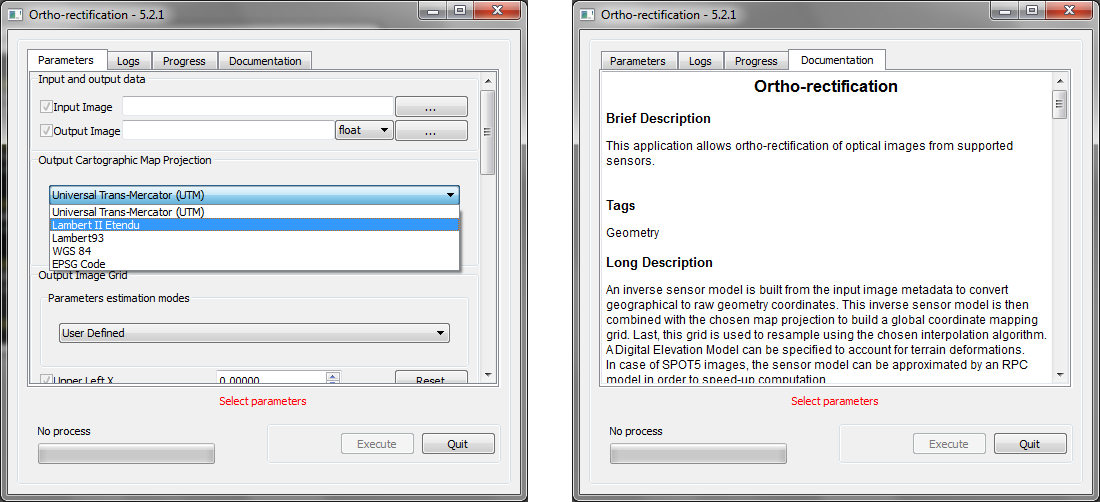
\includegraphics[width=1\textwidth]{images/otbgui.png}
\end{center}
\end{frame}

\begin{frame}[fragile]
\frametitle{Applications: appel depuis l'interface Python}
\begin{lstlisting}[language=python,breaklines=true,breakatwhitespace=true,frame = tb,framerule = 0.25pt,fontadjust,backgroundcolor={\color{listlightgray}},basicstyle = {\ttfamily\tiny},keywordstyle = {\ttfamily\color{listkeyword}\textbf},identifierstyle = {\ttfamily},commentstyle = {\ttfamily\color{listcomment}\textit},stringstyle = {\ttfamily},showstringspaces = false,showtabs = false,numbers = none,numbersep = 6pt, numberstyle={\ttfamily\color{listnumbers}},tabsize = 2]
#!/usr/bin/python

# Import the otb applications package
import otbApplication

# The following line creates an instance of the OrthoRectification application
OrthoRectification = otb.Registry.CreateApplication("OrthoRectification")

# The following lines set all the application parameters:
OrthoRectification.IO.IN = "QB_TOULOUSE_MUL_Extract_500_500.tif"
OrthoRectification.IO.OUT = "QB_Toulouse_ortho.tif"

app.MAP = 'epsg'
app.MAP.EPSG.CODE = 32768

# The following line execute the application
OrthoRectification.ExecuteAndWriteOutput()
\end{lstlisting}
\end{frame}


\begin{frame}
\frametitle{Monteverdi (accès aux applications OTB)}
\begin{minipage}[t][6cm][t]{\textwidth}
\begin{center}
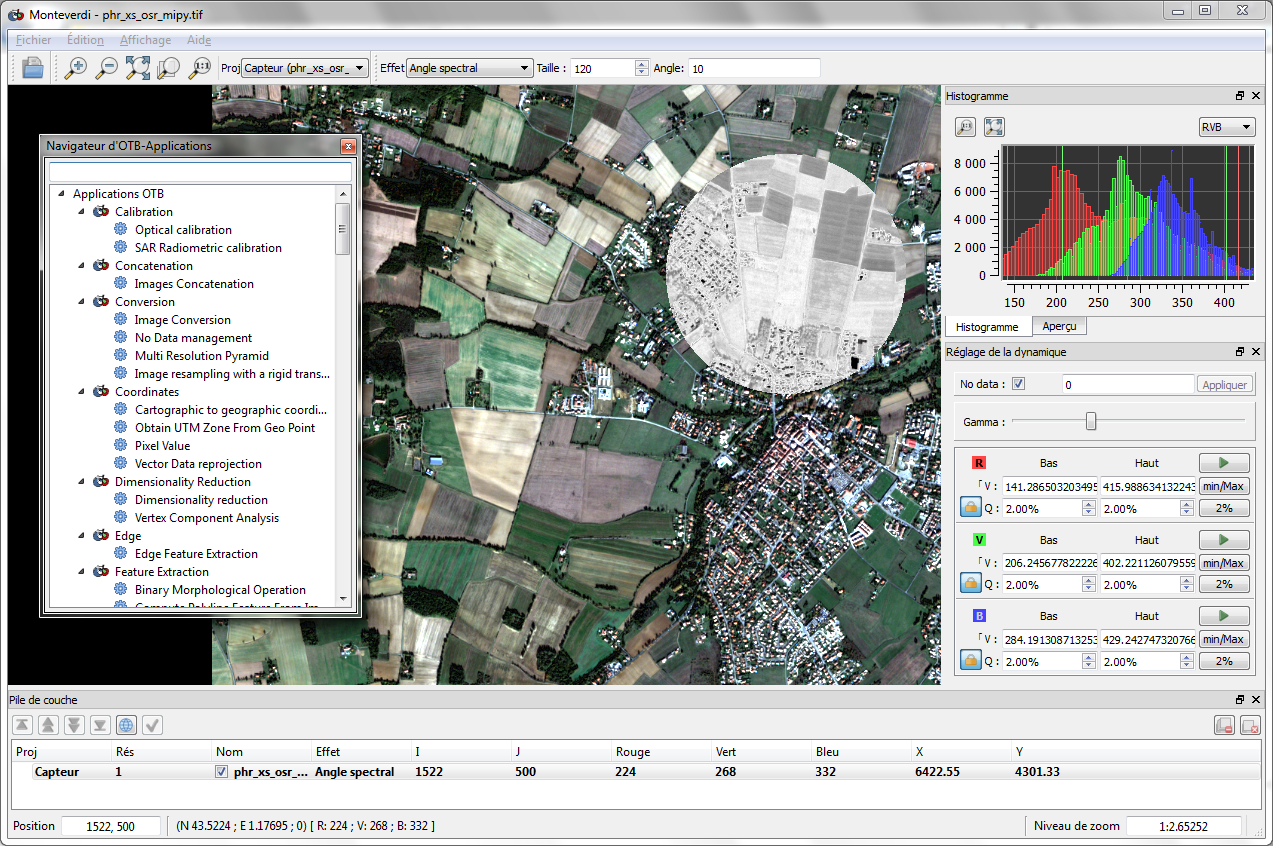
\includegraphics[width=1.0\textwidth]{images/monteverdi.png}
\end{center}
\end{minipage}
\end{frame}

%\vspace*{-3.0mm}
\begin{frame}
  \frametitle{QGIS (accès aux applications OTB)}
\begin{minipage}[t][6cm][t]{\textwidth}
\begin{center}
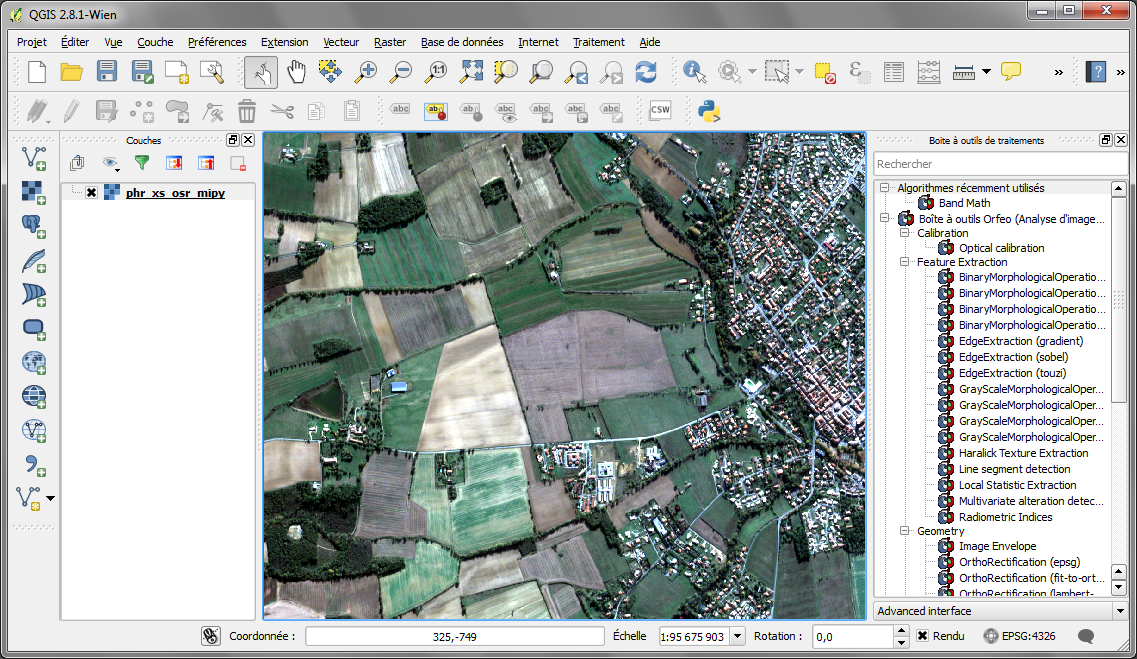
\includegraphics[width=1\textwidth]{images/otb_in_qgis.png}
\end{center}
\end{minipage}
\end{frame}

\begin{frame}
  \frametitle{Applications OTB ``as a service'' avec ZOO Project WPS}
\begin{minipage}[t][6cm][t]{\textwidth}
\begin{center}
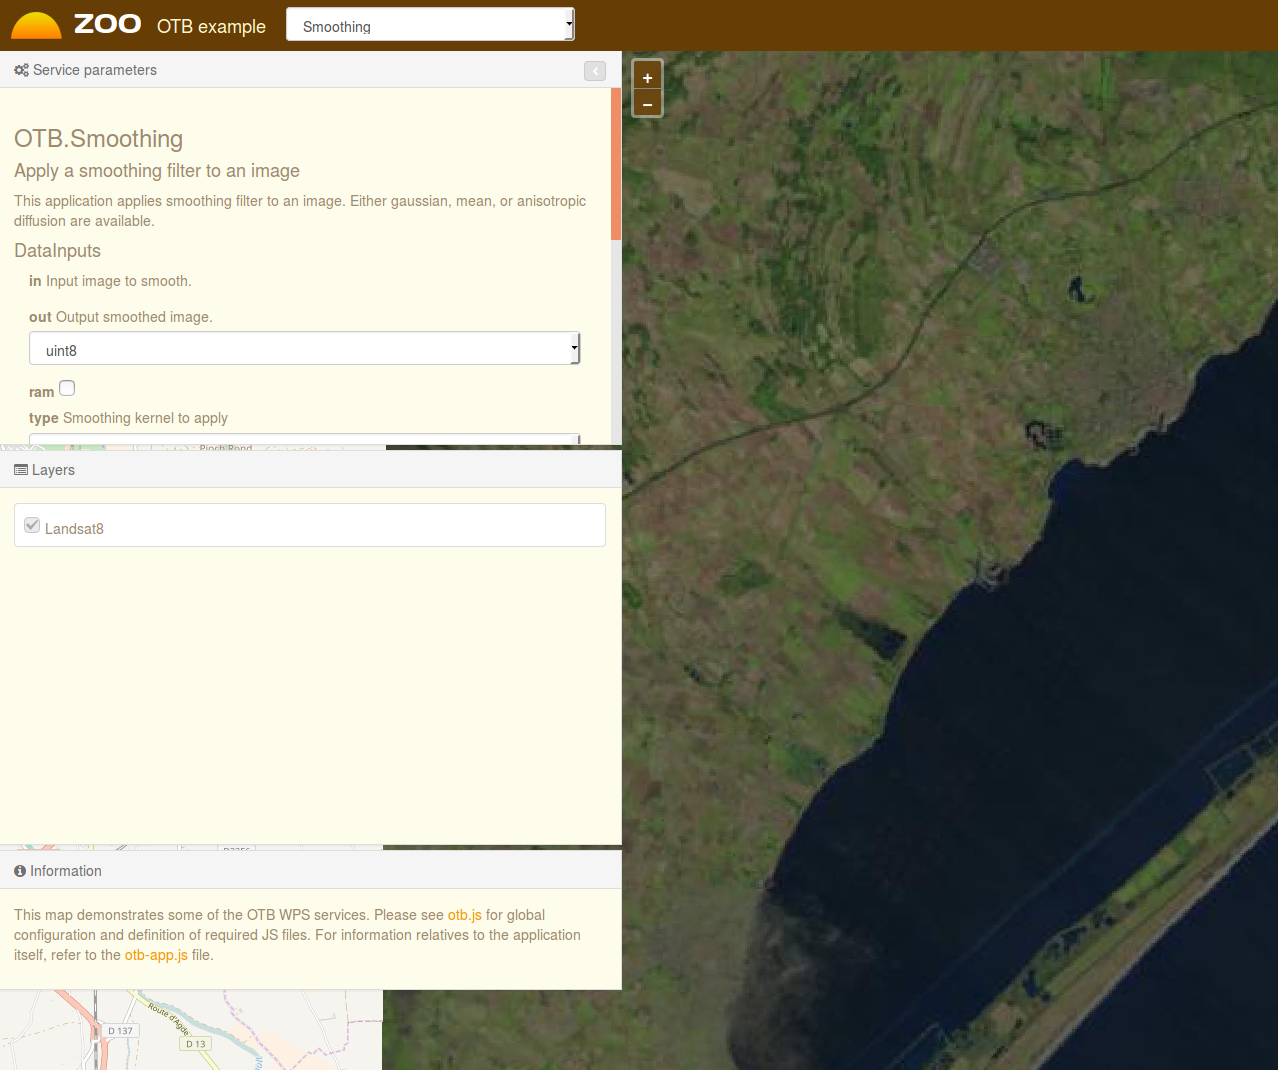
\includegraphics[width=0.7\textwidth]{images/otb_in_zoo.png}
\end{center}
\end{minipage}
\end{frame}

\section{Quoi de neuf depuis 5.0?}

\begin{frame}
\frametitle{5.0 (Mai 2015)}
\begin{block}{Modularité}
\begin{itemize}
\item Une meilleure organisation du code, en modules cohérents (124 modules et
    16 groupes) contenants sources, tests et applications.
\item Gestion des dépendances
\item Contributions externes: \url{https://www.orfeo-toolbox.org/external-projects/}
\end{itemize}
\end{block}

\begin{block}{SuperBuild}
\begin{itemize}
\item Il n'y a plus de logiciels tiers dans l'OTB
\item Le Superbuild, télécharge, configure, compile et installe les dépendances
\item Il existe également un mode \textit{offline} pour compiler l'OTB sans
  accès internet (en avion par exemple).
\end{itemize}
\end{block}
\end{frame}

\begin{frame}
\frametitle{Gouvernance ouverte: Project Steering Committee}
\begin{block}{Genèse du PSC}
  \begin{itemize}
  \item Jusqu'en 2015: l'OTB, un logiciel à sources ouvertes
  \item En mars 2015: l'OTB devient un logiciel libre, le CNES nomme un PSC initial
  \end{itemize}
\end{block}
\begin{block}{Un club de développeurs, pas de décideurs}
  \begin{itemize}
  \item Pilotage haut niveau du projet, roadmaps, communication, planification
  \item Vote les RFCs: Tous les membres ont le même poids dans les votes ($\pm 1$, $\pm 0$)
  \item Les sièges n'expirent pas, sortie par démission ou vote d'expulsion
  \item Le PSC n'est pas une entité légale et n'a pas de moyens propres
  \end{itemize}
\end{block}
\begin{block}{En chiffres}
  \begin{itemize}
  \item 5 membres de 4 entités différentes
  \item 2 release sous l'égide du PSC (5.2, 5.4)
  \item 3 meetings en ligne (logs publics)
  \end{itemize}
\end{block}
\end{frame}

\begin{frame}
\frametitle{5.2 (Décembre 2015)}
\begin{block}{OTB}
\begin{itemize}
\item Nouvelles applications pour le traitement SAR (polarimétrie, radiométrie, speckle)
\item Support des produits Sentinel-1 (calibration radiométrique)
\item Amélioration accès OTB en Python
\item Compatibilité avec GDAL 2.0 et support des images Sentinel-2
\item \ldots
\end{itemize}
\end{block}

\begin{block}{Monteverdi 3.0}
\begin{itemize}
\item Affichage mosaïque d'images ou série multi-temporelle
\item Outils de visualisation performants (contraste local, gradient\ldots)
\item Accès aux applications OTB
\end{itemize}
\end{block}
\end{frame}

\begin{frame}
\frametitle{5.4 (Mai 2016)}
\begin{block}{OTB}
\begin{itemize}
\item Passage à un cycle de release fixe (3 mois)
\item Intégration du composant de visualisation
\item Compilation externe des modules externes
\item Nouvelles décompositions SAR: Barnes, Huynen, Pauli
\end{itemize}
\end{block}

\begin{block}{Monteverdi 3.2}
\begin{itemize}
\item Capture d'écran
\item Génération d'overviews GDAL
\item Gestion des sous datasets GDAL
\item Ajout au SuperBuild
\end{itemize}
\end{block}
\end{frame}

\begin{frame}
\frametitle{5.6 (August 2016)}
\begin{block}{OTB}
\begin{itemize}
\item Parallélisation de l'exécution du pipeline avec la librairie MPI
\item Extraction et sélection d'échantillons pour la classification supervisée
\item Amélioration de la classification données vecteurs
\item Support des images Sentinel-1 (calibration géométrique)
\end{itemize}
\end{block}

\begin{block}{Monteverdi 3.4}
\begin{itemize}
\item Amélioration affichage et accès aux OTB applications
\end{itemize}
\end{block}
\end{frame}

\begin{frame}[fragile]
\frametitle{Parallélisation de traitements OTB avec MPI}
\begin{center}
  \vspace{-0.5cm}
  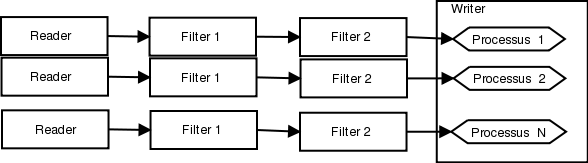
\includegraphics[width=0.6\textwidth]{images/mpi.png}
  \begin{scriptsize}
\begin{verbatim}
    $ mpirun -np $nb_procs --hostfile $PBS_NODEFILE  \
    otbcli_BundleToPerfectSensor \
    -inp $ROOT/IMG_PHR1A_P_001/IMG_PHR1A_P_201605260427149_ORT_1792732101-001_R1C1.JP2 \
    -inxs $ROOT/IMG_PHR1A_MS_002/IMG_PHR1A_MS_201605260427149_ORT_1792732101-002_R1C1.JP2 \
    -out $ROOT/pxs.tif uint16 -ram 1024

    ------------ JOB INFO 1043196.tu-adm01 -------------
    
    JOBID           : 1043196.tu-adm01
    USER            : michelj
    GROUP           : ctsiap
    JOB NAME        : OTB_mpi
    SESSION         : 631249
    RES REQSTED     : mem=1575000mb,ncpus=560,place=free,walltime=04:00:00
    RES USED        : cpupercent=1553,cput=00:56:12,mem=4784872kb,ncpus=560,vmem=18558416kb,
    walltime=00:04:35
    BILLING         : 42:46:40 (ncpus x walltime)
    QUEUE           : t72h
    ACCOUNT         : null
    JOB EXIT CODE   : 0
    
    ------------ END JOB INFO 1043196.tu-adm01 ---------
\end{verbatim}
\end{scriptsize}
\end{center}
\end{frame}

\begin{frame}
\frametitle{5.8 (Octobre 2016)}
\begin{block}{OTB}
\begin{itemize}
\item Implémentation Random Forest de Shark: plus performante, apprentissage parallèle
\item Meilleure performances BandMathX
\item Support spot7 (calibration radiométrique et géométrique)
\item Connection en mémoire des applications
\item Finalisation  du nouveau framework de classification
\item Et plein d'autres petites améliorations ...
\end{itemize}
\end{block}

\begin{block}{Monteverdi}
\begin{itemize}
\item Intégration aux sources de l'Orfeo ToolBox
\item Zoom avec molette sans CTRL
\end{itemize}
\end{block}
\end{frame}

\begin{frame}
  \frametitle{5.10 (février 2017)}
  \begin{block}{OTB}
    \begin{itemize}
      \item Framework pour applications composites
      \item Refactoring TrainImagesClassifier et BundleToPerfectSensor (composite)
      \item Affichage de la ligne de commande correspondante dans les GUI QT des applications
      \item Amélioration du composant de sélection des champs dans les GUI QT
      \item Application FFT/DWT
      \item Calcul des textures de Haralick sous échantillonnées (release majeure)
    \end{itemize}
  \end{block}
  
  \begin{block}{Monteverdi}
    \begin{itemize}
      \item Pseudo-couleur à bande unique
      \end{itemize}
  \end{block}
      
\end{frame}

\begin{frame}
  \frametitle{6.0 (mai 2017)}
  \begin{block}{OTB}
    \begin{itemize}
      \item Changement de licence pour Apache v2.0
      \item Support OpenCV 3.0
      \item Application pour deburst des produits Sentinel1 IW SLC
      \item Sélection des bandes par noms de fichier étendus
      \item Classification non-supervisée intégrée au framework
      \item Application pour profils morphologiques
      \item Application pour classer des vecteurs
      \item Nettoyage des fonctions dépréciées
    \end{itemize}
    \end{block}
\end{frame}

\begin{frame}
  \frametitle{6.2 (Octobre 2017)}
  \begin{block}{OTB}
    \begin{itemize}
      \item Amélioration des messages d'erreurs, de la documentation des applications
      \item Application de segmentation \textit{all in one}
      \item Amélioration applications: Convert, DownloadSRTMTiles, PixelValue, ExtractROI
      \item Paquets binaires inclus fichiers nécessaires pour développer avec l'OTB
      \item OTB est officiellement un logiciel OSGeo!
    \end{itemize}
    \end{block}
\end{frame}

\section{Conclusion et perspectives}
\begin{frame}
\frametitle{Combien d'utilisateurs ?}
\begin{columns}[c]
\column{0.5\textwidth}
\begin{block}{Difficile à dire \ldots}
\begin{itemize}
    \item $\approx$ 600 membres sur la liste utilisateurs
    \item $\approx$ Entre 100 et 150 messages par mois
    \item $\approx$ 100 membres sur la liste développeurs
    \item $\approx$ 118 comptes sur le système de gestion des bugs
    \item $\approx$ 50 contributeurs (listé dans la documentation)
    \item $\approx$ 3400 téléchargements for OTB 5.0
  \end{itemize}
\end{block}
\begin{block}{Users Days 2015, 2016 et 2017}
  15 à 20 participants à Toulouse pendant 3 jours
\end{block}
\column{0.5\textwidth}
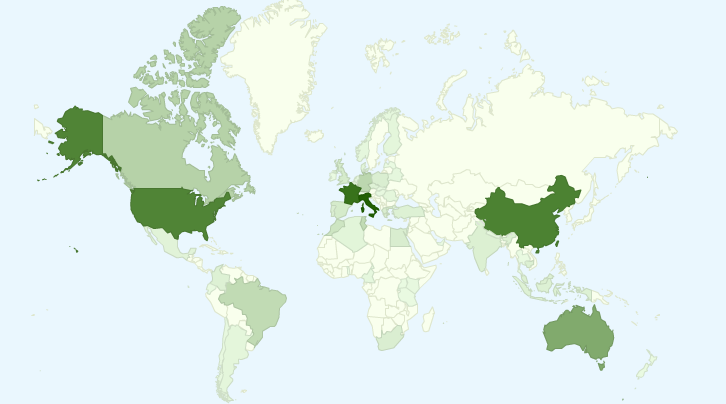
\includegraphics[width=0.9\textwidth]{images/OTB4_download_sourceforge_country_crop.png}\\
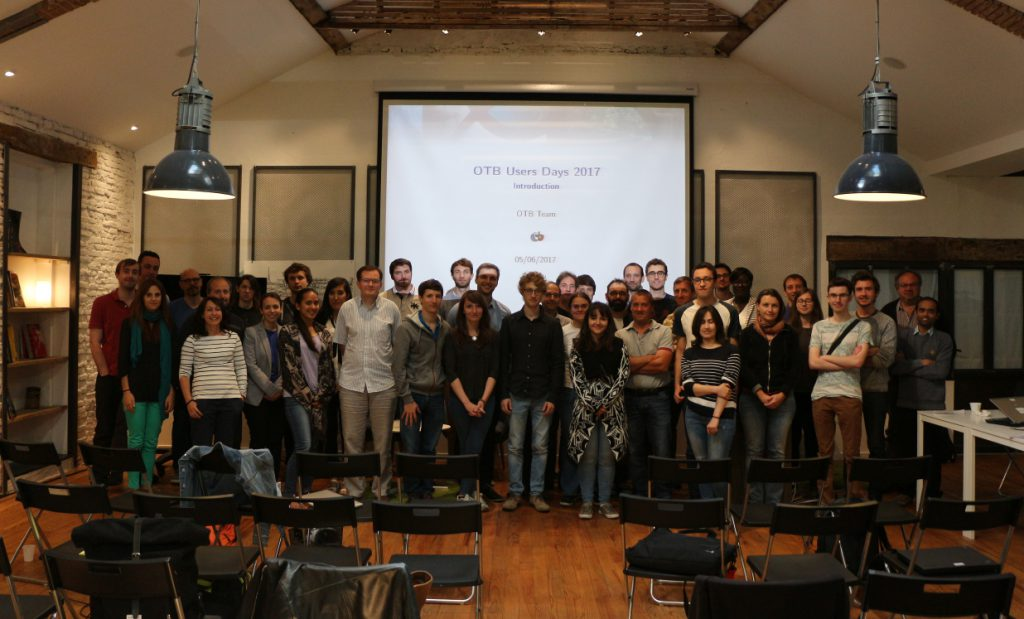
\includegraphics[width=0.9\textwidth]{images/userdays2017.jpg}
\end{columns}

\end{frame}

\begin{frame}
\frametitle{Les réussites de l'OTB}
\vspace{-0.5cm}
\begin{columns}
\column{0.65\textwidth}
\begin{itemize}
\item l'OTB a été utile à (certains) des utilisateurs ORFEO!
\item L'OTB a traité avec succès plus de 619 images Pléiades pour le site web RTU,
\item L'OTB fournit beaucoup de fonctions utiles pour la télédétection dans un \textbf{unique outil}
\item L'OTB est (a été) l'unique logiciel open-source compatible avec les images Pléiades (grâce à OpenJPEG)
\item L'OTB égale ou dépasse les outils de l'état de l'art (libre et commercial) pour certaines fonctions:
\begin{itemize}
\item La calculatrice de bandes,
\item La segmentation de scène complètes,
\item La classification à l'échelle d'une scène complète avec un grand choix d'algorithmes,
\item Les ponts entre la télédétection et le systèmes d'information géographique\ldots
\end{itemize}
\item Au delà d'ORFEO, l'OTB est déjà utilisée dans plusieurs projets et logiciels
\end{itemize}
\column{0.35\textwidth}
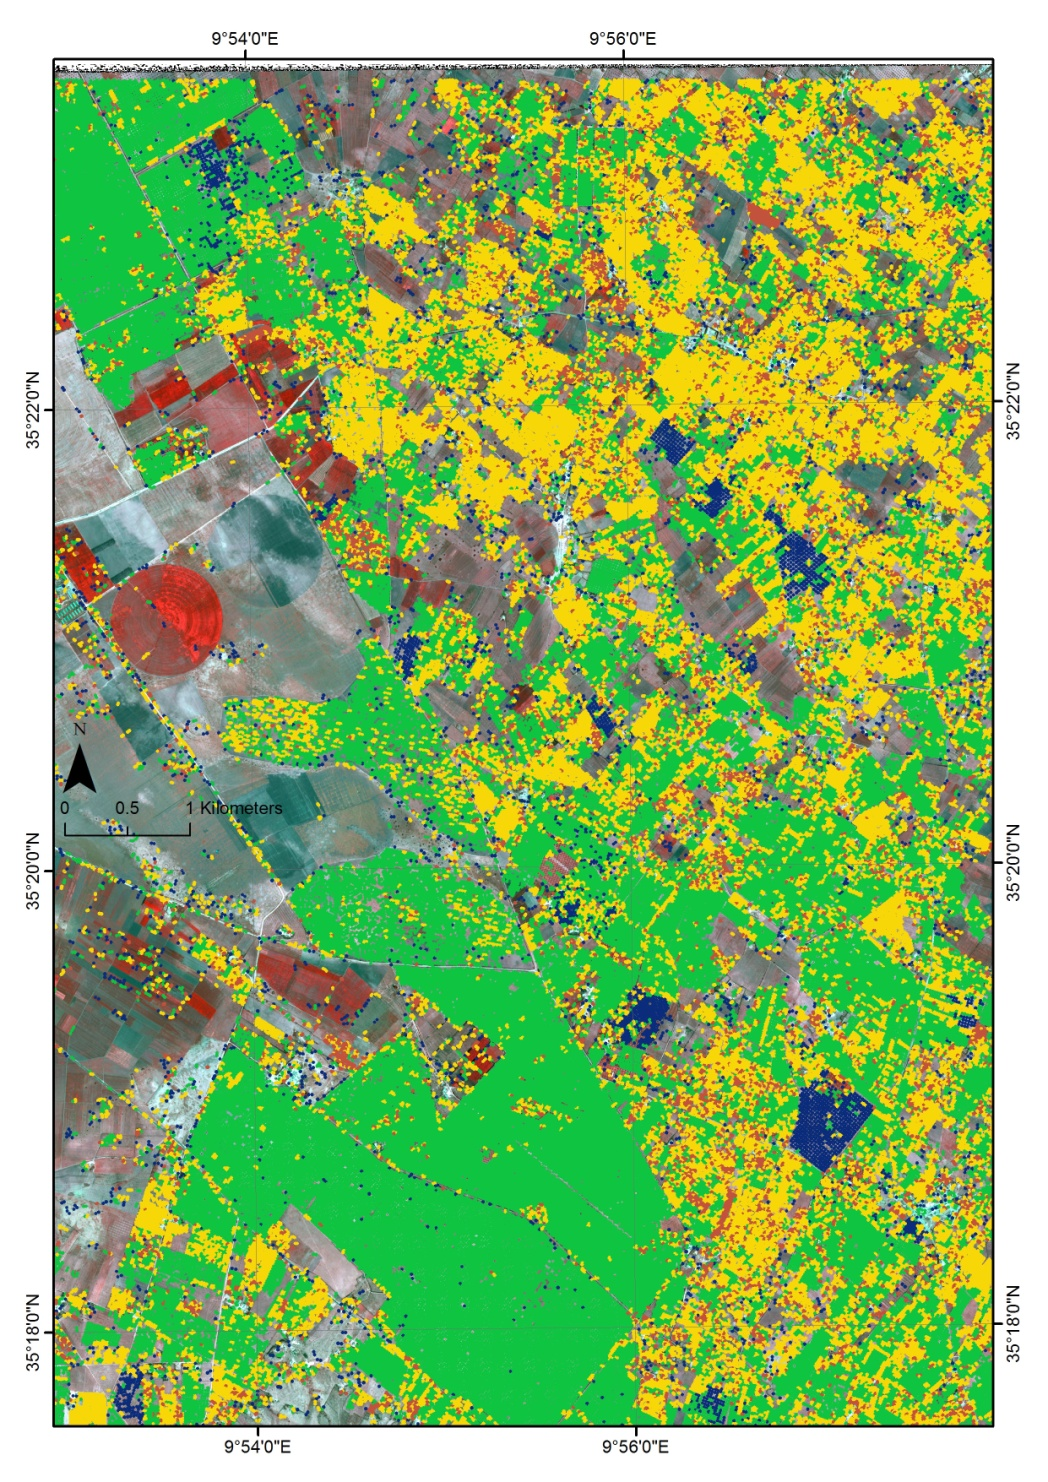
\includegraphics[width=0.9\textwidth]{images/resultats_ird.png}\\
\tiny{Carte thématique à partir d'une segmentation par l'OTB, B. Mougenot~-~IRD}
\end{columns}
\end{frame}

\begin{frame}
  \frametitle{Projets et logiciels utilisant l'OTB}
  \vspace{-0.5cm}
\begin{columns}
  \column{0.55\textwidth}
  \begin{itemize}
    \item Les applications OTB applications sont disponibles dans le module de traitement de QGIS
    \item Support dans Zoo-Project (service WPS)
    \item L'OTB est utilisée dans certains composant des segments sols S2 et
      Venus (CNES et ESA)
    \item Logiciel éducatif Terr'Image
    \item Utiliser pour générer des produits à l'échelle nationale en France
      dans THEIA
    \item Projet EA S2 Agriculture
    \item Le logiciel Gnorasi (National Technical University of Athens)
    \item Projet GEOSUD (IRSTEA)
    \item Le programme de recherche TCM (ETS Quebec)
  \end{itemize}
  \column{0.6\textwidth}
\begin{center}
  \includegraphics[width=0.6\textwidth,height=0.35\textheight]{images/Carte_17Classes.png}\\
  \tiny{Produit occupation du sol THEIA (CESBIO)}
  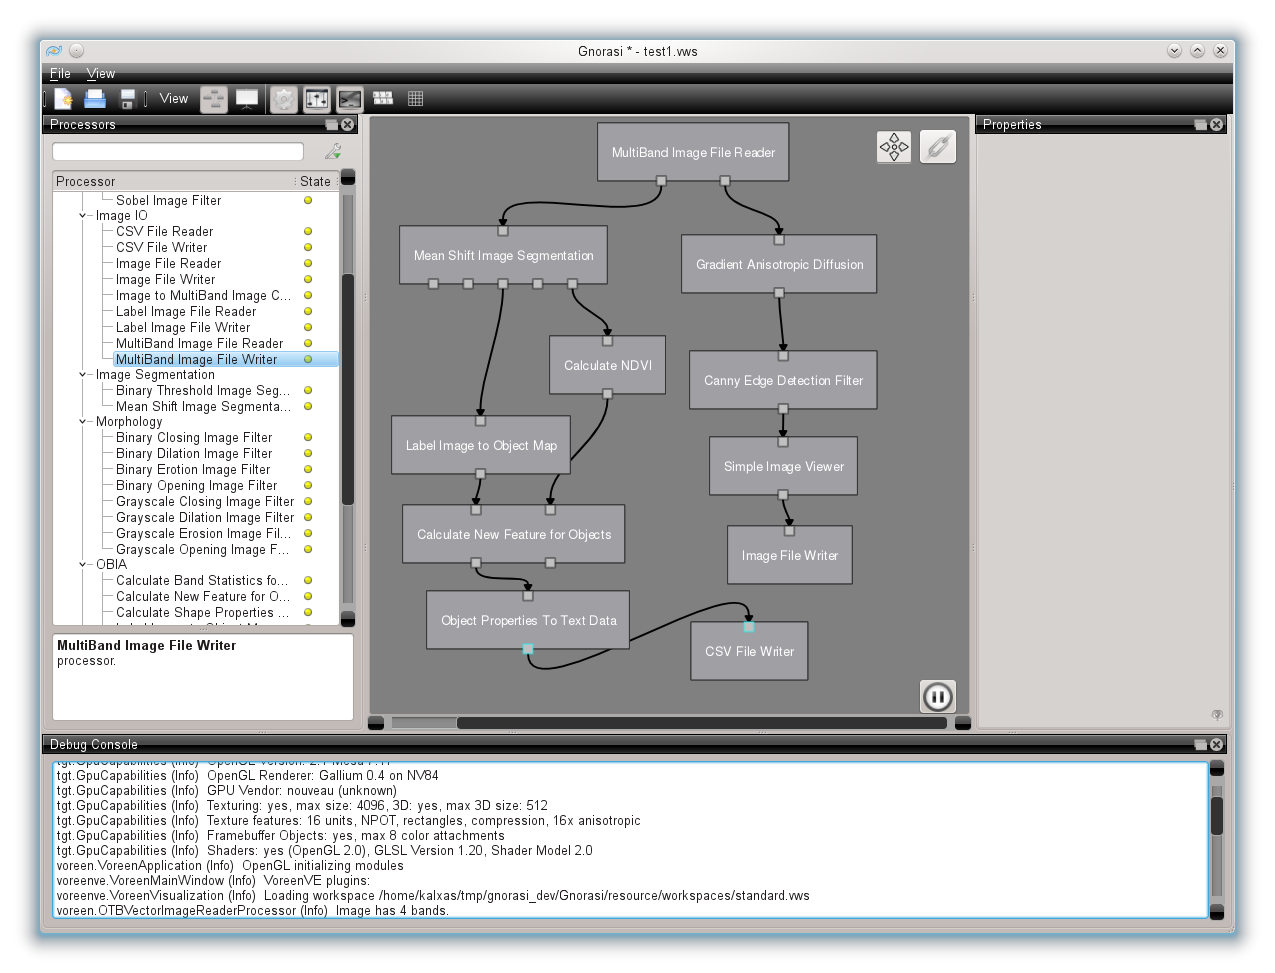
\includegraphics[width=0.6\textwidth]{images/gnorasi2.png}\\
  \tiny{Le logiciel Gnorasi}
\end{center}
\end{columns}
\end{frame}

\begin{frame}
\frametitle{Support/Aide/Contribution}
\vspace{-0.2cm}
\begin{block}{Ressources}
\vspace{-0.2cm}
\begin{description}
\item[Site web] \href{http://www.orfeo-toolbox.org}{orfeo-toolbox.org}
\item[Wiki] \href{http://wiki.orfeo-toolbox.org}{wiki.orfeo-toolbox.org}
\item[Blog] \href{http://blog.orfeo-toolbox.org}{blog.orfeo-toolbox.org}
\end{description}
\end{block}
\vspace{-0.2cm}
\begin{block}{Documentation et aide}
\vspace{-0.2cm}
\begin{description}
\item[Doxygen] \href{http://www.orfeo-toolbox.org/doxygen/}{doxygen}
\item[Documentation] Software Guide et CookBook (remote sensing recipes)
\item[Liste de diffusion utilisateurs] otb-users@googlegroups.com
\item[Liste de diffusion développeurs] otb-developers@googlegroups.com
\end{description}
\end{block}
\vspace{-0.2cm}
\begin{block}{Follow-up}
\vspace{-0.2cm}
\begin{description}
\item[Code, bugs, contributions, feature requests \ldots] \href{https://gitlab.orfeo-toolbox.org/orfeotoolbox/otb}{gitlab.orfeo-toolbox.org}
\item[Météo?] \href{http://dash.orfeo-toolbox.org}{dash.orfeo-toolbox.org}
\end{description}
\end{block}
\end{frame}

\begin{frame}
\frametitle{Merci pour votre attention. Des questions?}
\begin{minipage}[t][6cm][t]{\textwidth}
\begin{center}
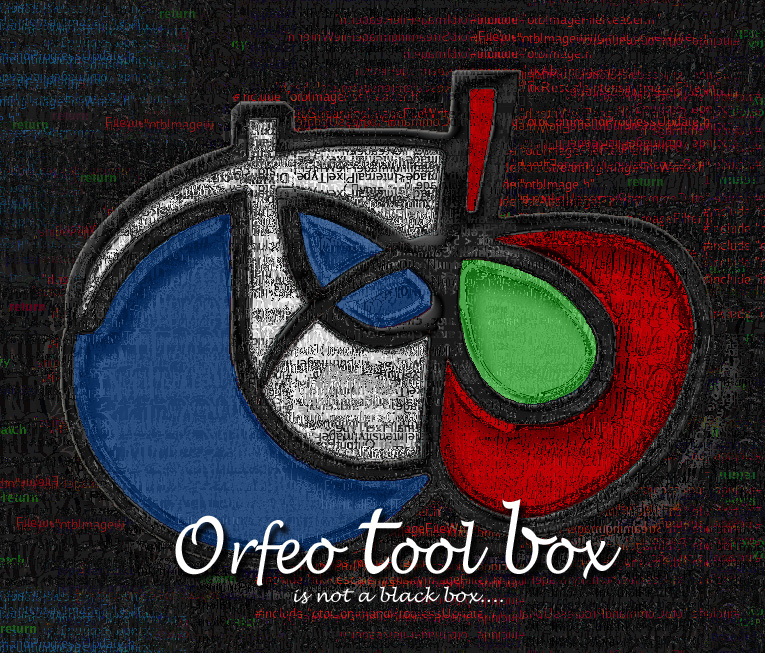
\includegraphics[width=0.65\textwidth]{images/LOGOTB_blackbox.png}
\end{center}
\end{minipage}
\end{frame}

\end{document}
